\documentclass{beamer}

\input{../Vor2017glærur}

\title{Tölvunarfræði 2}
\subtitle{Vika 8}

\begin{document}

\begin{frame}
\titlepage
\end{frame}

\section{Inngangur}

\begin{frame}{Skoðanakönnun úr síðasta tíma}
\begin{center}
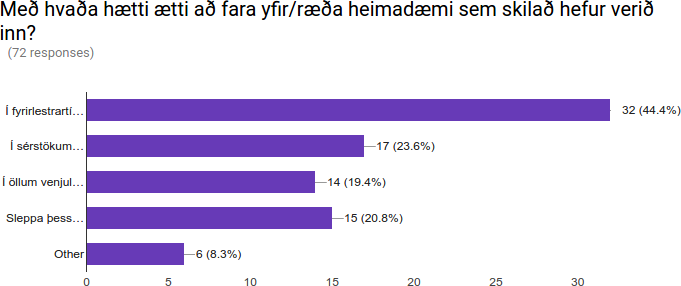
\includegraphics[width=\textwidth]{poll-results}
\end{center}
Í samræmi við niðurstöður - ræðum skil 7 undir lok tímans
\end{frame}


\begin{frame}{Upprifjun: Tré}
\begin{columns}
\column{0.6\textwidth}
\begin{itemize}
 \item Algengt er í tölvunarfræði að raða gögnum upp í tré
 \item Hugmyndin eins og við munum nota hana:
 \begin{itemize}
  \item Höfum hnúta, hver hnútur inniheldur vísun í tvö eða fleiri \emph{börn}
  \begin{itemize}
   \item Vísunin getur verið tóm
  \end{itemize}
  \item Getum kallað hnút sem er ekki barn neins annars \emph{rót}, hnút sem á engin ekki-tóm börn \emph{lauf}
 \end{itemize}
 \item Sértilvik: tvíundartré \eng{binary tree}, þar sem barnafjöldinn er 2
\end{itemize}
\column{0.4\textwidth}
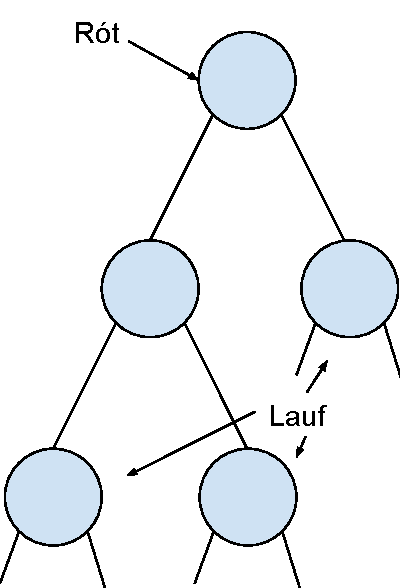
\includegraphics[width=\linewidth]{tree-example}
\end{columns}
\end{frame}


\section{Hrúgur}

\begin{frame}{Hrúgur}
Hrúga \eng{heap} er tvíundartré sem uppfyllir hrúguskilyrði \eng{heap property}. Við notum fylki til að geyma hrúgur.

Skoðum glærur 16-17 í \href{http://algs4.cs.princeton.edu/lectures/24PriorityQueues.pdf}{PriorityQueues}.
\end{frame}

\begin{frame}{Aðgerðir}
\begin{itemize}
 \item Notkun hrúgu til að útfæra forgangsbiðröð krefst tveggja aðgerða
 \item Innsetning
 \begin{itemize}
  \item Setjum stakið aftast og látum það synda upp
 \end{itemize}
 \item Eyðing stærsta staks
 \begin{itemize}
  \item Skiptum á rót og síðasta stakinu í fylkinu, sökkvum því sem við færðum upp
 \end{itemize}
 \item Skoðum glærur 20-23 í \href{http://algs4.cs.princeton.edu/lectures/24PriorityQueues.pdf}{PriorityQueues}.
\end{itemize}
\end{frame}

\begin{frame}{Tími}
\begin{itemize}
 \item Athugum - um fullskipuð tré er að ræða
 \item Innsetning og eyðing felur í sér færslu á milli hæða í trénu
 \item Fjöldi aðgerða takmarkast af hæð trésins
 \begin{itemize}
  \item Hæð fullskipaðs trés með $N$ hnútum er $\lfloor \log_2 n \rfloor$
 \end{itemize}
 \item Praktísk vandræði við útfærsluna eins og henni hefur verið lýst er að langt er á milli staka, hentar illa fyrir minnisuppbyggingu raun
\end{itemize}
\end{frame}

\section{Minnisuppbygging tölva}

\begin{frame}{Minnisuppbygging}
\begin{columns}
\column{0.6\textwidth}
\begin{itemize}
 \item Sumir geymslustaðir fyrir gögn eru hraðvirkari en aðrir
 \item Gróf uppbygging í nútímatölvu:
 \begin{enumerate}
  \item Minni örgjörvans \eng{internal memory} - gisti \eng{registers} og skyndiminni \eng{cache}
  \item Aðalminni \eng{main memory}  - RAM
  \item Aukageymsla \eng{secondary storage} - SSD diskar/harðir diskar
  \item Útvær geymsla \eng{off-line storage} - geymsla utan stjórnar örgjörvans
 \end{enumerate}
\end{itemize}
\column{0.4\textwidth}
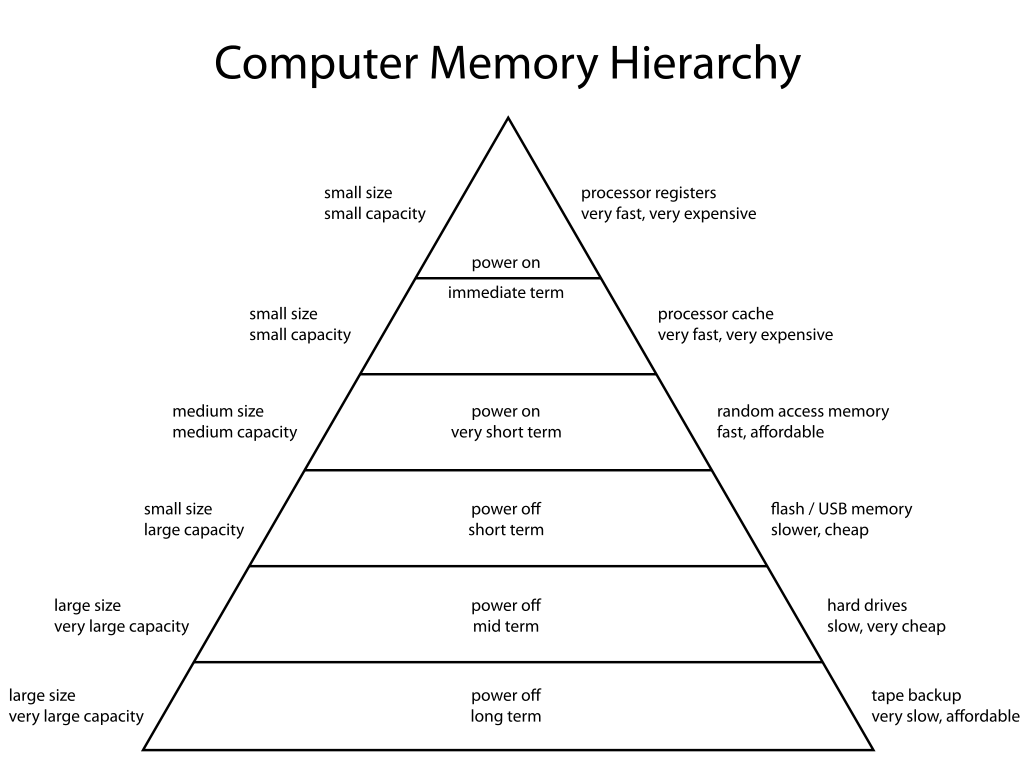
\includegraphics[width=\linewidth]{computer-memory-hierarchy}
\begin{center}
\href{https://en.wikipedia.org/wiki/Memory\_hierarchy}{Mynd af Wikipedia}
\end{center}
\end{columns}
\end{frame}

\section{Nafnatöflur}

\begin{frame}{Nafnatöflur}
\begin{columns}
\column{0.5\textwidth}
\begin{itemize}
 \item Nafnatafla \eng{symbol table} er mjög almenn hugræn gagnagrind
 \item Snýst um að tengja saman lykla (e. \emph{keys}) og gildi (e. \emph{values})
 \begin{itemize}
  \item ``Hvert er gildið fyrir þennan lykil?''
 \end{itemize}
 \item Höfum þegar séð útfærslu á nafnatöflu - \texttt{std::map} í C++
\end{itemize}
\column{0.5\textwidth}
\begin{center}
DNS tafla
\begin{tabular}{cc}
\toprule
Lykill&Gildi\\
\midrule
mbl.is&92.43.192.110\\
visir.is&82.221.81.10\\
hi.is&130.208.165.207\\
ru.is&52.48.55.82\\
\bottomrule
\end{tabular}
\end{center}
\end{columns}
\end{frame}

\begin{frame}{API}
Möguleg skil fyrir nafnatöflu:
\begin{center}
\begin{tabularx}{\textwidth}{rlX}
\toprule
\multicolumn{3}{c}{\texttt{public class ST<Key, Value>}}\\
\midrule
-&\texttt{ST()}& Smiður, býr til tóma nafnatöflu\\
\texttt{void}&\texttt{void put(Key k, Value v)}&Setja lykil-gildis par í töfluna\\
\texttt{Value}&\texttt{get(Key key)}&Skilar gildinu sem svarar til \texttt{key}\\
\bottomrule
\end{tabularx}
\end{center}
Auk þess mætti skilgreina \texttt{delete(Key key)}, \texttt{contains(Key\ key)}, \texttt{size()} og \texttt{isEmpty()} aðferðir
\end{frame}

\begin{frame}{Útfærsla á nafnatöflu}
\begin{itemize}
 \item Við gætum sett gögnin okkar í óraðað fylki eða eintengdan lista
 \begin{itemize}
  \item Sjá: \href{http://algs4.cs.princeton.edu/code/edu/princeton/cs/algs4/SequentialSearchST.java.html}{SequentialSearchST.java}
  \item Verður tímafrekt fyrir stórar töflur
 \end{itemize}
 \item Getum notað öflugri aðferðir ef við getum gert ráð fyrir meiru um lyklana
 \begin{itemize}
  \item Viljum hafa lykla sem eru samanburðarhæfir (sjá \texttt{Comparable})
  \item Seinna: Lykla sem hægt er að taka af \texttt{hashCode}
 \end{itemize}
 \item Almennt ráðlagt: Nota óbreytanlega \eng{immutable} lykla
 \begin{itemize}
  \item Gott: \texttt{Integer}, \texttt{String}, \texttt{Double},\ldots
  \item Slæmt: T.d. fylki
 \end{itemize}
\end{itemize}
\end{frame}

\section{Helmingunarleit}

\begin{frame}{Helmingunarleit}
\begin{itemize}
 \item Hingað til höfum við notað línulega leit til að finna staðsetningar í fylkjum og listum
 \item Getum gert betur í röðuðum fylkjum, hugmyndin er:
 \begin{itemize}
  \item Berum ``miðju'' leitarbilsins saman við leitarstakið
  \item Sé miðjan stærri en leitarstakið vitum við að stakið er ekki að finna í stærri helming leitarbilsins (og öfugt)
  \item Notum helmingunarleit endurkvæmt á þann helming leitarbilsins sem eftir er
 \end{itemize}
 \item Leitaraðferðin er kölluð helmingunarleit \eng{binary search} því hún helmingar stærð leitarbilsins í hverri ítrun
 \item Grundvallaraðferðafræði sem kemur víða við!
 \item Skoðum \href{http://algs4.cs.princeton.edu/code/edu/princeton/cs/algs4/BinarySearchST.java.html}{BinarySearchST.java} vandlega
\end{itemize}
\end{frame}

\begin{frame}{Endurkvæm helmingunarleit}
\begin{center}
Möguleg endurkvæm útfærsla á helmingunarleit:

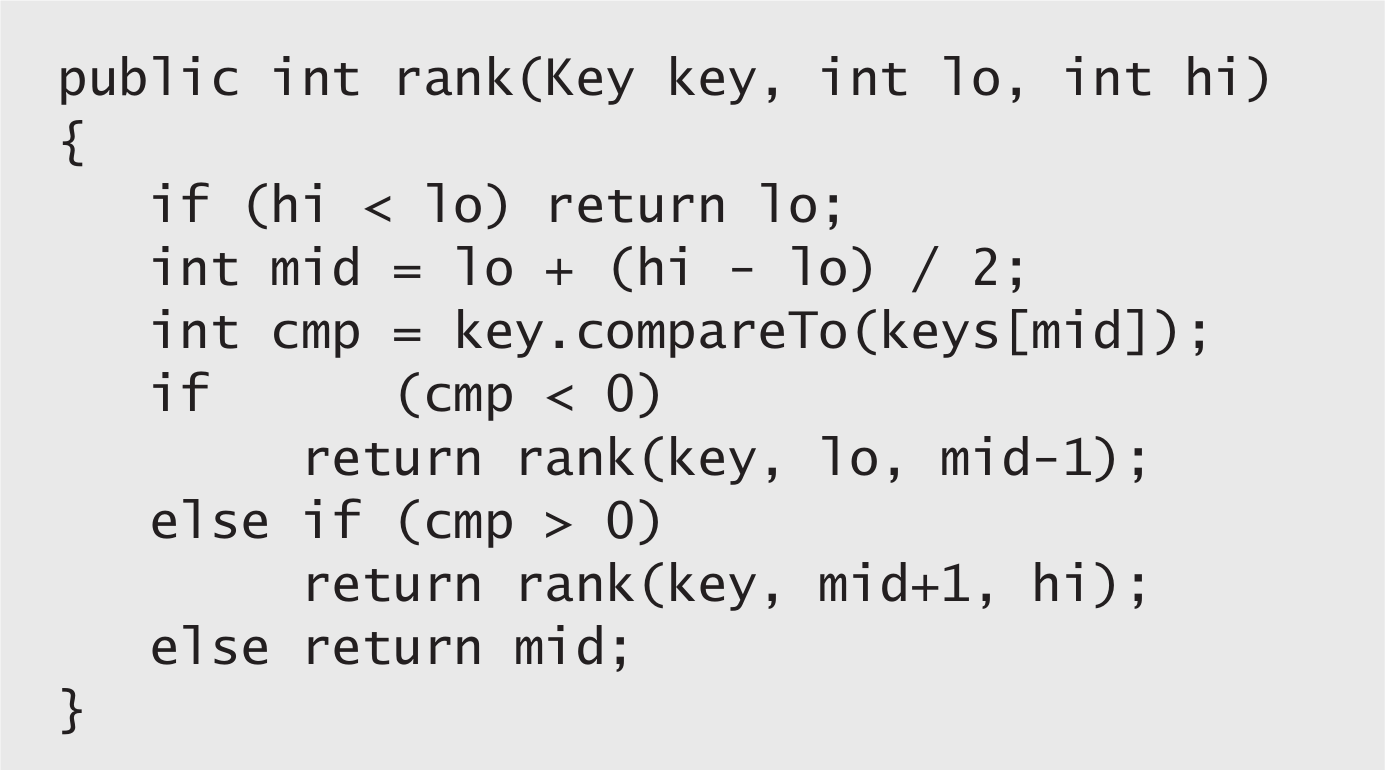
\includegraphics[width=0.7\textwidth]{binary-search-algs4-380}
\end{center}
Sjá bls. 380 í Algorithms.
\end{frame}


\begin{frame}{Tími}
\begin{itemize}
 \item Getum lýst fjölda samanburða í helmingunarleit í $N$ staka fylki með rakningarvenslum:
 \begin{itemize}
  \item $C(0) = 0$, $C(1) = 1$ , $C(N) = C(\lfloor N \rfloor)+1$
  \item Fáum $C(N) \sim \log N$
 \end{itemize}
 \item Útfærslan á nafnatöflunni í \texttt{BinarySearchST.java} leyfir skilvirkar uppflettingar (logratími)
 \item Innsetningar og eyðingar krefjast hins vegar enn línulegs tíma
\end{itemize}
\end{frame}

\section{Tvíleitartré}

\begin{frame}{Tvíleitartré}
\begin{itemize}
 \item Við getum auðveldað helmingunarleit með því að geyma gögnin í tvíundartré
 \begin{itemize}
  \item Í þetta skiptið - táknað með hnútum og bendum, líkt og við höfum gert þegar við höfum útfært eintengda lista
 \end{itemize}
 \item Til að útfæra nafnatöflu látum við hnúta innihalda samanburðarhæfan lykil, notum uppbyggingu trésins til að auðvelda leitina
 \begin{itemize}
  \item Látum vinstra barn hvers hnúts hafa minni lykil en hnúturinn, hægra barnið stærri lykil
 \end{itemize}
 \item Köllum þessi tvíundartré tvíleitartré \eng{binary search tree}
 \item Skoðum nafnatöflu útfærða með tvíleitartré, \href{http://algs4.cs.princeton.edu/code/edu/princeton/cs/algs4/BST.java.html}{BST.java}
\end{itemize}
\end{frame}

\begin{frame}{Aðgerðir á tvíleitartré}
\begin{itemize}
 \item Til að uppfylla skil fyrir nafnatöflu þurfum við að geta:
 \begin{itemize}
  \item Leitað eftir lykli (\texttt{get})
  \begin{itemize}
   \item Berum leitarlykilinn saman við lykil hvers hnúts
   \item Förum í vinstra eða hægra undirtré eftir hvern samanburð
   \item Hættum þegar lykillinn finnst eða þegar við finnum \texttt{null}
  \end{itemize}
  \item Innsetning (\texttt{put})
  \begin{itemize}
   \item Svipað og leit, en þegar við finnum \texttt{null} setjum við stakið inn
  \end{itemize}
 \end{itemize}
 \item Sjá glærur 4-10 í \href{http://algs4.cs.princeton.edu/lectures/32BinarySearchTrees.pdf}{BinarySearchTrees}
 \item Eyðing er kafli út af fyrir sig (sjá glærur 31-34 í BinarySearchTrees)
\end{itemize}
\end{frame}

\begin{frame}{Þessi glærupakki}
Tengill á fyrirlestraræfingu: \url{https://goo.gl/forms/xgWGlDlmEvGlbcu93}
\vspace{1cm}

Kóða fyrir algs4 reiknirit má finna á \url{http://algs4.cs.princeton.edu/code/}
\end{frame}

\begin{frame}{Næst}
Meira um tvíleitartré, hakkatöflur.
\end{frame}



\end{document}
